% Insert as a new results subsection before Limitations.
% Copy fig/rsr_classical.pdf into the manuscript's fig directory.
% Source: results/p1_revision/reused/rsr_and_noise_summary.json.
% These 2,800 stored worlds are from sahure_expansion, not the original
% 27,300-trial Paper 1 verification. No new Monte Carlo worlds were drawn.

\subsection{Effect of Reference Strength}
\label{sec:revision-rsr}

We also test how the reference strength affects the benefit of the Hankel
constraint. We use $N=32$, $K=3$, $P=30$, SNR $=5$~dB, and independently
sampled path counts $L_k\in\{3,\ldots,7\}$. The single-user RSR takes
the values $0$, $5$, $10$, $12$, $15$, $20$, and $25$~dB. Both estimators
use 100 final updates. HS-GS uses 25 updates per candidate rank, four
Cadzow sweeps per application, and the same 30\% validation split followed
by a final fit using all pilots.

This supplementary analysis reuses 2,800 stored paired trials from a
separate simulation campaign, with 400 trials at each RSR. These are
distinct from the original 27,300 trials reported above. No new Monte
Carlo realizations were generated for this analysis. We use only the
classical EM-GS and HS-GS results. Pointwise 95\% confidence intervals
use 4,000 paired bootstrap resamples.

Fig.~\ref{fig:revision-rsr} shows that HS-GS improves on EM-GS at all
seven RSR values in this experiment. The ratio-of-sums gain ranges from
$1.83$ to $2.51$~dB, and each corresponding confidence interval is above
zero. At RSR $=0$~dB, the gain is $1.83$~dB, with a 95\% interval of
$[1.40,2.26]$~dB. The paired-median gain at this point is $2.83$~dB;
these are different summaries of the same paired errors.

The weak reference still makes channel estimation harder for both
methods. At RSR $=0$~dB, the EM-GS and HS-GS NMSEs are $-6.19$ and
$-8.01$~dB. At RSR $=12$~dB, they are $-10.73$ and $-12.93$~dB.
Thus, the structural gain remains useful at the weakest tested reference,
but it does not remove the loss caused by that weak reference. The gain
does not increase steadily with RSR. These findings apply to the tested
array size, SNR, and channel distribution.

\begin{figure*}[!t]
\centering
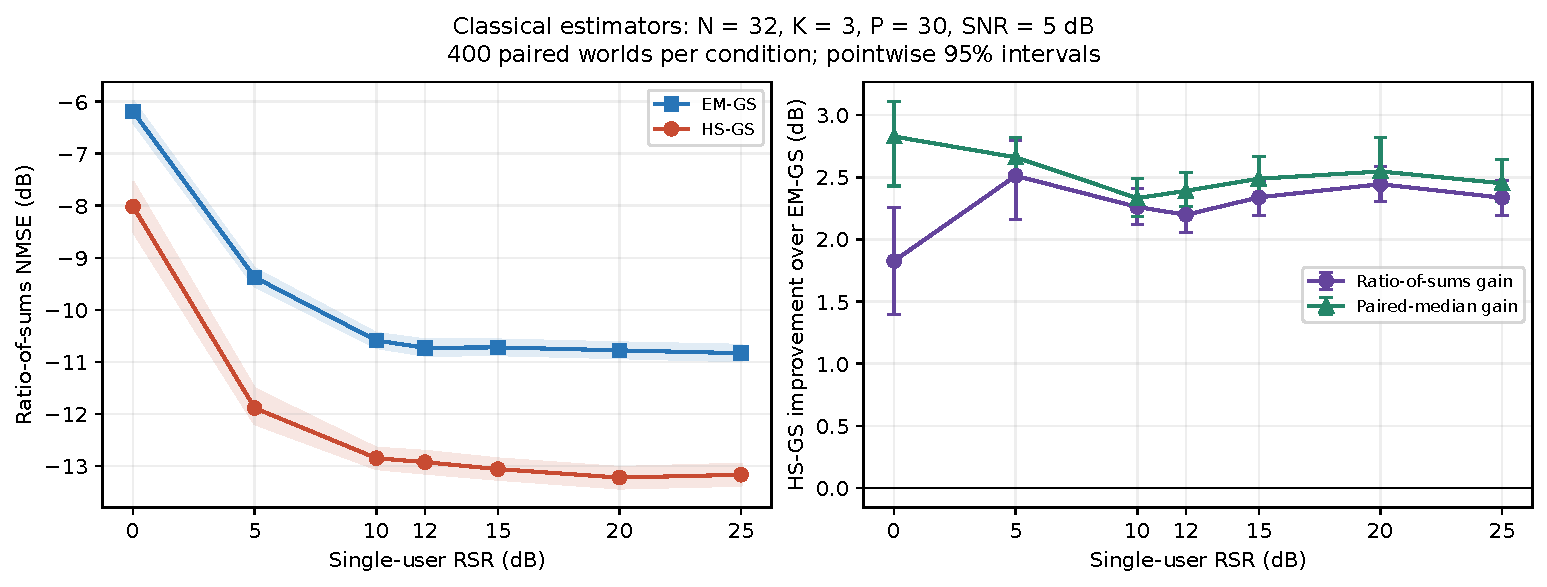
\includegraphics[width=\textwidth]{fig/rsr_classical.pdf}
\caption{Effect of single-user RSR for $N=32$, $K=3$, $P=30$, and
SNR $=5$~dB. Left: ratio-of-sums NMSE. Right: HS-GS gain measured by the
ratio of summed errors and by the paired median. Shaded bands and error
bars are pointwise 95\% paired-bootstrap intervals. Each RSR uses 400
paired trials from a separate stored campaign.}
\label{fig:revision-rsr}
\end{figure*}
